\documentclass{article}
\usepackage{tikz}
\usetikzlibrary{shapes.geometric,calc,angles,positioning,intersections,quotes,decorations,babel,patterns,fit}
\usepackage{tkz-euclide}
\usetkzobj{all}
\begin{document}
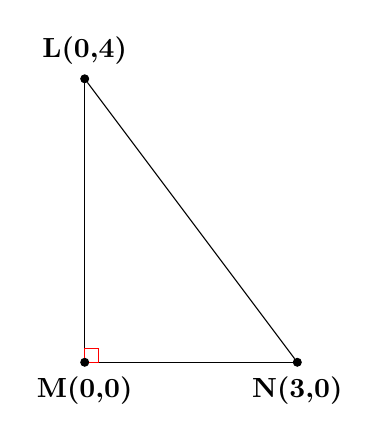
\begin{tikzpicture}
[scale =0.9,>=stealth,point/.style = {draw, circle, fill = black, inner sep = 1pt},]
\node (L) at (0,4)[point,label=above :$\textbf{L(0,4)}$] {};
\node (M) at (0,0)[point,label=below :$\textbf{M(0,0)}$] {};
\node (N) at (3,0)[point,label=below :$\textbf{N(3,0)}$] {};

\draw (L)--(M);
\draw (M)--(N);
\draw (L)--(N);

\tkzMarkRightAngle[draw=red,size=.2](L,M,N)
 
\end{tikzpicture}
\end{document} 